\section{Motivation and introduction}
\blindtext[1]
\section{Materials and methods}
\blindtext[1]
\subsection{IMDB dataset}
\blindtext[1]
\subsection{Feature engineering}
In order to properly understand the data and see the performance of models in later stages, feature engineering is an important step that must be performed initially to ensure that irregularities are not negatively affecting the performance.
\subsubsection{Rescraping}
First step in this project was to scrape the data again. The original dataset had a lot of missing values for many features, including some important ones, like budgets, so scraping process was  repeated in order to fill those gaps, or to regenerate the dataset. The process was done in three stages, by modifying the original parsing script to solve the shortcomings of the original dataset. 

First, up to date budget values were taken from website that has a database of production and marketing budgets for movies (thenumbers.com), as well as domestic and worldwide gross values. The original dataset only included the domestic gross estimates from IMDB.com, which are severely lacking and for majority of popular films omit large portions of revenue that was earned in other countries. As the worldwide gross is the target value that was being predicted, and ultimately that measured the success of the models presented, it was important to get this part right.

Second, based on list of movies obtained from first step, script obtained the IMDB links for the movies, using fuzzy matching (as some movies have several names that identify them, eg. Fast \& Furious 6 and Furious 6) to resolve naming ambiguities, and parsed the available data about genre, actors, year and other important features. In this step the script queried the Facebook for popularity measures, count of likes, for actors, movies and director.

Finally, third step was to join the data from all steps in a single dataset, ordered by highest grossing movies, in a machine readable csv file. Other than the resolving most of the missing values and updating the information, main contribution of this step was the correct worldwide gross values. Additionally, all values were converted to a common currency (USD), as in the original dataset this was not the case. This was heavily influenced some Korean and Chinese movies that had billions in revenue, due to the exchange rate of their currency compared to USD.
\subsubsection{Data cleaning}
After obtaining the updated and improved dataset, additional work was performed manually to clean and enhance the data. Duplicates were removed, and additional columns were added, like ‘blockbuster’, which designated is the movie released during Christmas or Summer season (June/July/August/December), as well as manual fixing of duration, countries, and similar values that show outliers. Some movies, for example, has a length of close to 10 hours, and all these tasks were performed by OpenRefine.

\subsubsection{Categorisation}
Additionally, other techniques were applied to account for the variety of data types as well as large ranges of values. Given that the ranges for the worldwide gross are several orders of magnitude, from hundreds of thousands of dollars, all the way to billions, logarithmic transform can be applied to minimise the range effect.

Polynomial.

Finally, categorisation of the data was performed to handle the textual fields and increase the count of features. Most popular directors, actors, as well as binary features (like colour) were transformed to categories, so in the end resulting dataset had significantly more features that the original dataset.
\subsection{Exploratory data analysis (EDA)}
Exploratory data analysis was applied after the dataset was collected, processed and cleaned, with the purpose of understand the nature of the data, the relationships between the variables, and discover patterns that can guide the selection and application of prediction machine learning techniques \cite{behrens1997principles}. Since our goal is to predict the success of a movie before the premiere day, we are specially interested in the variables that could tell us if a movie is going to be successful or not. One of such variables is the “worldwide gross” or “box-office”.  FIGURE(a) shows that the gross variable is exponentially distributed. Therefore it could be useful to use the logarithmic transformation to deal with a more normally distributed version of this variable. The result of the logarithmic transformation of this variable is shown in FIGURE(b). A similar exploration was applied on the gross variable, which is probably one of the best explanatory variables for measuring the success of a movie. 


Gross 

(b) Logarithmic transformation of the Gross
FIGURE: Histograms of the gross variable


(a) Budget

(b) Logarithmic transformation of the budget
FIGURE: Histograms of the budget variable

FIGURE presents a scatter plot of the two variables discussed previously in their original form and in the log transformed form. Both plots indicate a linear relationship between the budget and the gross variable, however the data distribution is heteroscedastic, which could suggest the use of a Weighted Least Squares (?). 


(a) Gross versus budget

(b) log(gross) versus log(budget) 


FIGURE: Scatter plot of the gross versus the budget

We extended the bivariate data analysis to other variables by means of a correlation matrix and a pairwise plot. These graphical tools are presented in FIGURE and FIGURE. From FIGURE it can be seen that as expected gross and budget are correlated (Correlation coefficient=0.74). Unfortunately, there is not a significant correlation between the movie gross and the other explanatory variables. 


FIGURE: Correlation matrix for the numeric features. 

\iffalse
Other observations (https://blog.nycdatascience.com/student-works/machine-learning/movie-rating-prediction/) taken from the correlation matrix:
The "cast_total_facebook_likes" has a strong positive correlation with the "actor_1_facebook_likes", and has smaller positive correlation with both "actor_2_facebook_likes" and "actor_3_facebook_likes"
The "movie_facebook_likes" has strong correlation with "num_critic_for_reviews", meaning that the popularity of a movie in social network can be largely affected by the critics
The "movie_facebook_likes" has relatively large correlation with the "num_voted_users"
The movie "gross" has strong positive correlation with the "num_voted_users"
'''
\fi


FIGURE: Plot pairwise relationships between selected features created with the seaborn python library.


\subsubsection{Dimensionality reduction}
The cumulative explained variance plot created by means of PCA over the processed dataset is shown in FIGURE, where it can be seen that there is not a small representative subset of variables that can explain the majority of variance in the data. In other words, 125 variables (out of 184) explain 80% of the variation. This means that there is not much space for dimensionality reduction in this dataset.

FIGURE: Explained variance plot.



Dimensionality reduction is also useful to create a visual representation of multidimensional data in a reduced space. For instance, FIGURE shows a PCA-reduced 3D representation of the dataset studied in this report. From FIGURE it can be drawn that most of the observations are scarcely scattered in a certain area of the plot, but also there is a considerable amount of points scattered outside that area. FIGURE also shows that there is not clear evidence of clusters. 

FIGURE: PCA-reduced 3D visualization of the dataset

\subsubsection{Approach}
The \textbf{pipeline} was built on top of sklearns Pipe and Gridsearch functions. It’s architecture was more advanced in comparison with original Pipe, as it supported a search of different models and not only the parameters.

We aim to find the most accurate model among different algorithms including regressions, logistic regression, random forest and neural net. For each model, we also need to set different values for each parameter in order to fine-tune the model.
 
Besides, before our data fed into the models, we performed numerous pretreatment methods towards the data, i.e. transformation, scaling and dimension reduction.
 
The workflows applied in this project is shown in figure1. In order to integrate and automate this workflows (excluding data collecting), we used a function called Pipeline in Scikit-learn, which allows us to set parameters for algorithms in each step while chaining them together without keeping track of the data.

\begin{figure}[h]
\centering
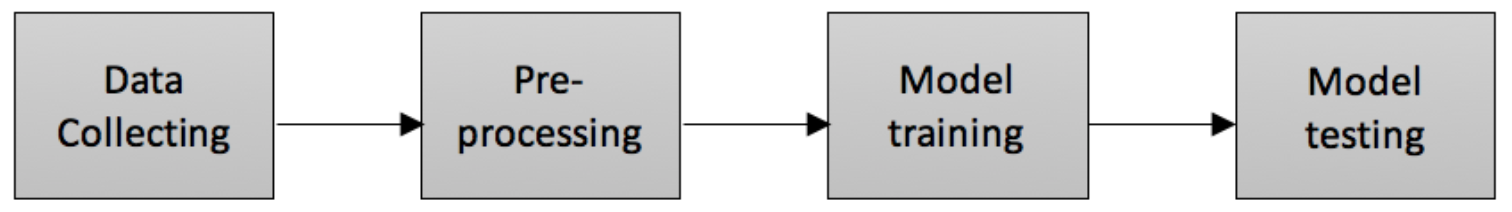
\includegraphics[width=3.2in]{figures/pipeline}
\caption{Pipeline diagram}
\label{fig:pipeline}
\end{figure}
 
However, each parameter in each model have different potential values and there are many different combinations of the parameters in between the workflows. All the values and combinations should be tested in order to find the most optimal one.
 
These processes of setting values and trying combinations can be tedious. GridSearchCV in Scikit-learn allows us to construct a grid of the combinations and search for the best one. Besides, it also automatically performs cross-validation on each model for each combination. In the end, it returns us with the best model and best parameters.

\textbf{Linear and Logistic Regressions:}
An ordinary linear regression model is a common starting point for analysis since its results can serve as a baseline for any further data analysis. The dependent variable, which is the movie gross, can be predicted using the multivariate linear regression. The highly correlatable predictors, such as number of facebook likes, IMBD score and number of reviews will be used to build a robust regression model. Later on, we can aggregate those factors by giving each of them a weight and then use below mentioned neural network technique to fine-tune the weights. Some other regression models, like k-nearest neighbour algorithm and multinomial logistic regression will be explored as well.

\textbf{Decision trees:}
Classification and Regression Trees (CART) trees could be another technique that apply in this case. Seeing as decision trees are able to handle both categorical and numerical data, there is the flexibility is drawing comparisons between both classification and regression.  Random Forests will also be considered in this case in order to add diversity to the decision tree models. 

\textbf{Neural Networks:}
Neural networks approach is useful in these types of problems where there is a lot of features, and based on data obtained from previous techniques, we will experiment with neural networks algorithms to see how they behave. Those include simpler neural networks, like feed-forward NN, to more complex ones, like recursive NN, which might show some additional insight.

By applying those techniques, we aim to build a successful model that accepts certain movie related factors and predicts the box-office and its rating. Additionally, we will compare the performance of the aforementioned machine learning techniques when predicting the box-office. We are also interested in assessing the performance of Ensemble Learning, which combines multiple models to cancel the systematic bias of individual forecast models. Gradient Boosting, an example of this approach, has proved to be effective in some of the last Kaggle competitions..
\section{Regression}
\subsection{Support Vector Machines}
\subsection{Neural networks}
\subsection{Gradient Boosting Regression}
Gradient Boosting was applied on the data, with least squares as the error function. The best result was produced with a Gradient Boosting Regressor with 1000 base learners and a corresponding low learning rate (0.1). Base learners in this case are decision trees which are used as weak learners in the gradient boosting process. These are constructed in a greedy fashion, choosing the best split to minimize the loss. 

Given the high number of regression trees combined to form the Gradient Boosting model, a visual inspection of individual trees is hard to interpret. We use the feature importance to highlight features that would ordinarily be used frequently in split points in our model. It is found that the most important features to the Gradient Boosting model are the production budget movie duration, and the total number of Facebook likes for the cast.  The production budget however immensely outweighs the other features in terms of importance. 

To extend this further, we take a look at partial dependence plots to show the dependence between the target response and the most important set of features (i.e. the expected response as a function of the features). Figure NN shows dependency plots for total number of Facebook likes, movie duration and production budget. The lower left plot shows the effect the production budget has on the movie gross, and it can be seen that there is a linear relationship (?) between them. 

The lower right plot shows the interactions among the production budget and movie duration, which are the two most important features as per the model. For a movie of a certain duration d (both high and low durations), its gross is strongly dependent on production budget.  The remaining two plots, point to the fact that there is not a strong linear relationship between the target variable and the Facebook likes of cast and movie duration.
\begin{figure}[h]
\centering
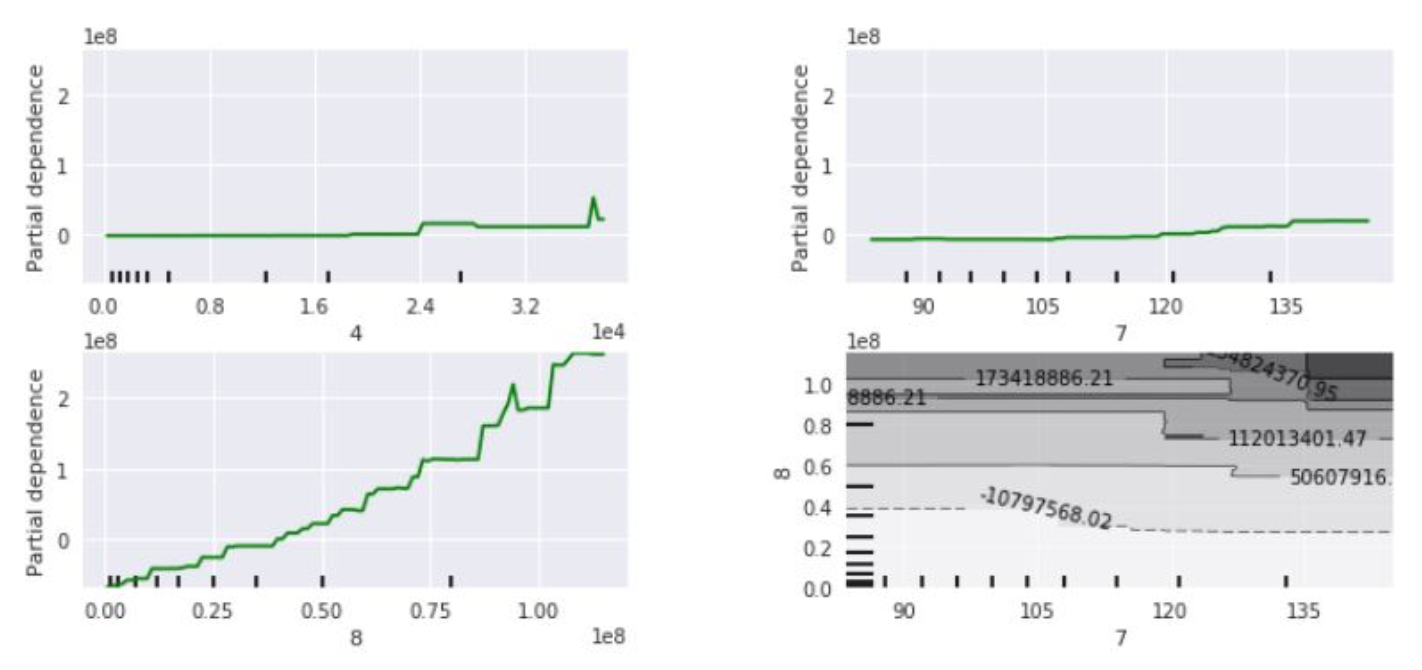
\includegraphics[width=3.2in]{figures/gradient_boost_dependency}
\caption{Dependency Plot for Gradient Boosting Model \cite{figgradientdep}}
\label{fig:figgradientdep}
\end{figure}
\section{Classification}
Over 20 different classifiers have been used within the pipeline. As result of experimentation pipeline had been narrowed down to 3 classifiers: Logistic Regression, Neural Networks and Gradient Boosting.

Gradient boosting regressor has been found to be the best performing classifier for all classification cases. This section discusses the parameters optimization for growing the decisions trees and constructing the ensembles to generalize a well fitted model, taking into account bias/variance trade-off [1].

\begin{figure}[h]
\centering
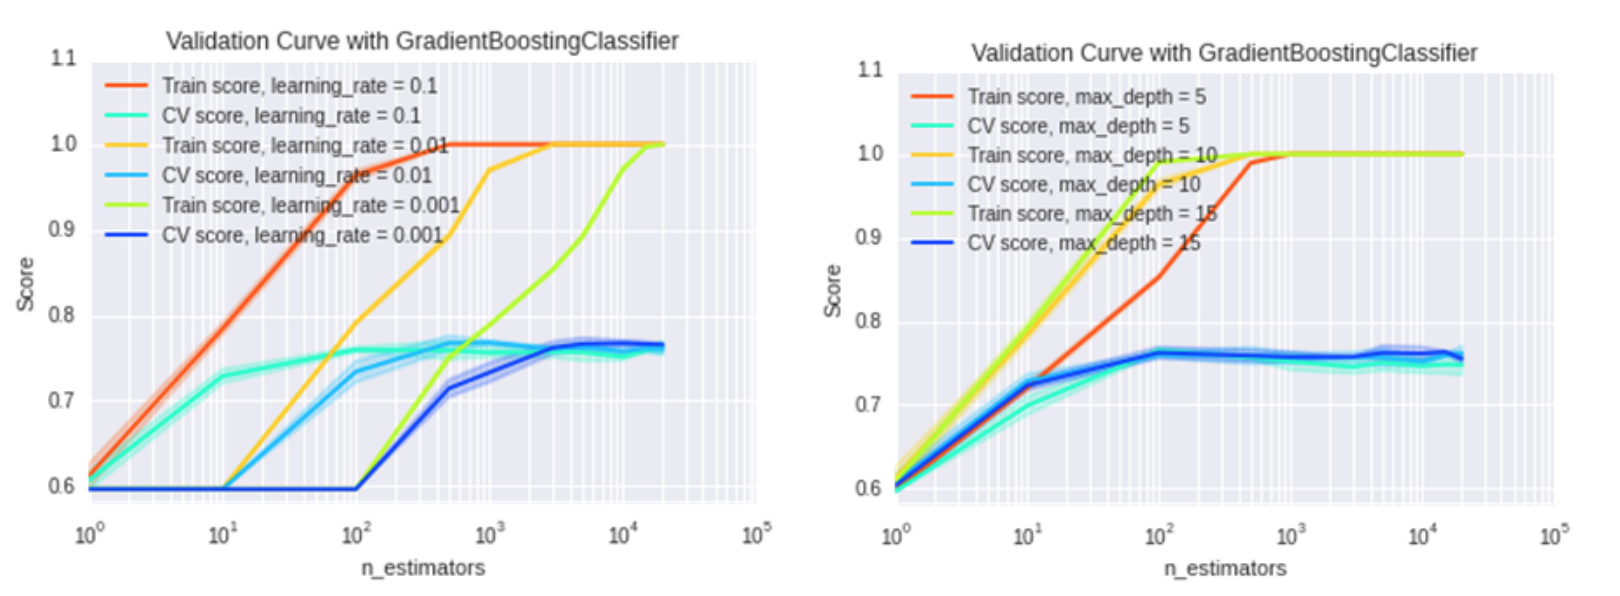
\includegraphics[width=3.2in]{figures/gb1}
\caption{GB1}
\label{fig:gb1}
\end{figure}
\begin{figure}[h]
\centering
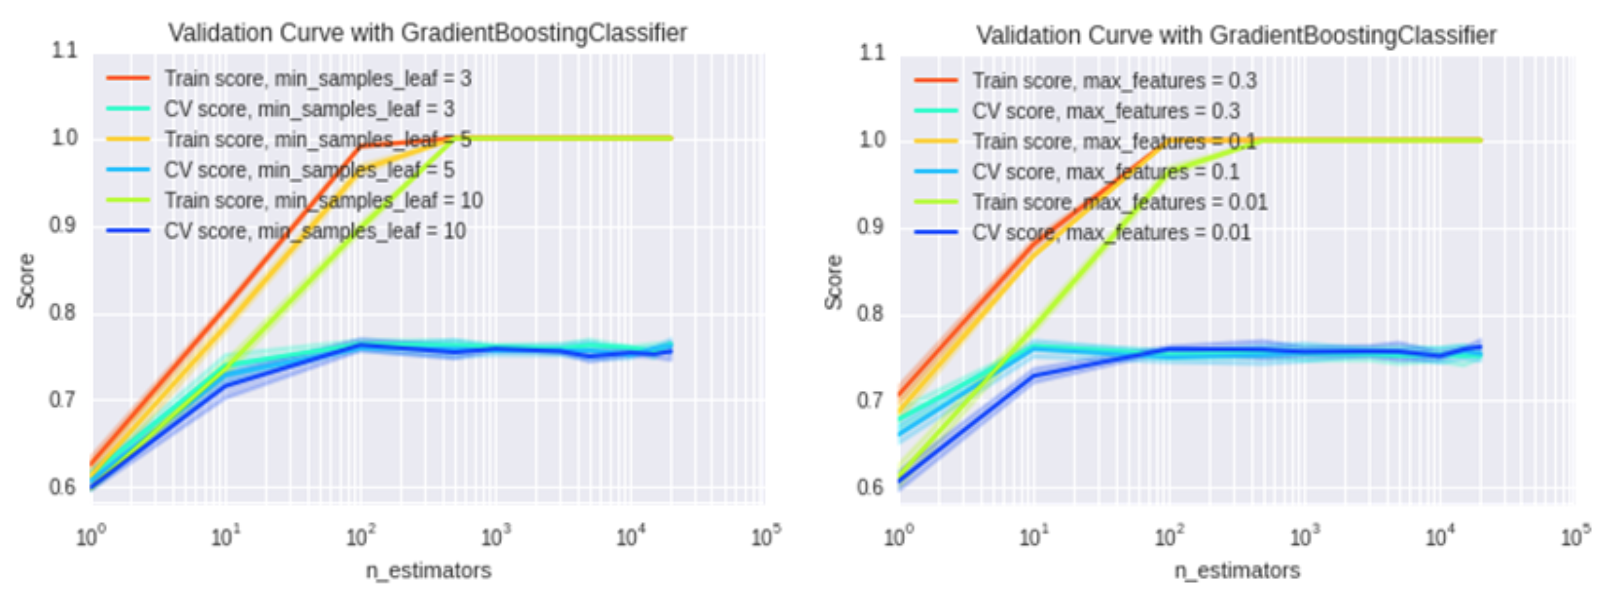
\includegraphics[width=3.2in]{figures/gb2}
\caption{GB2}
\label{fig:gb2}
\end{figure}
\begin{figure}[h]
\centering
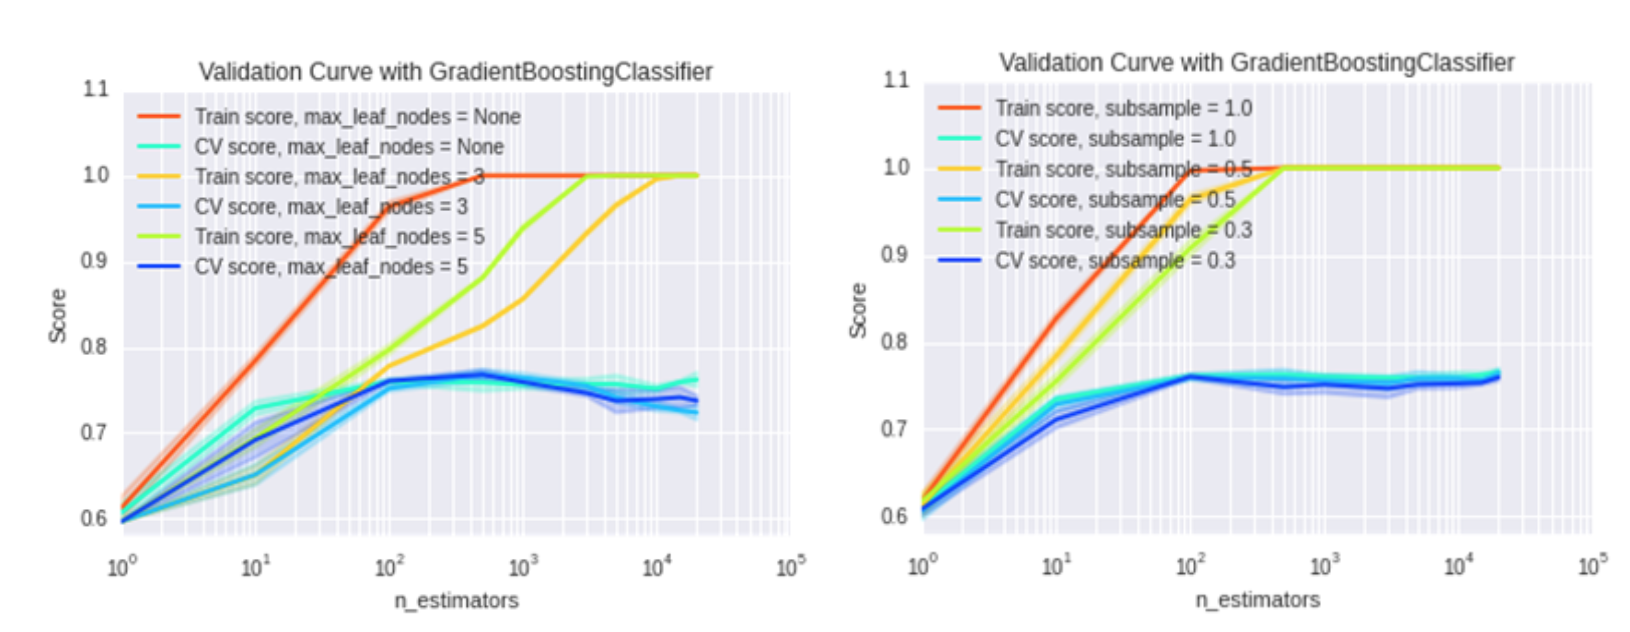
\includegraphics[width=3.2in]{figures/gb3}
\caption{GB3}
\label{fig:gb3}
\end{figure}

The learning rate/shrinkage represents the weight that is applied to the error minimization amount by each newly added decision tree [1]. As result a smaller learning rate requires more estimators to be added in order to more generalized model, as it can be seen in Figure 1. Learning rate of 0.01 achieves the highest performance with a small amount 500 ensembles and does not overcomplicate model as 0.001 rate. Max tree depth controls the maximal number of nodes within single tree, hence limiting number of decision a single tree can take. Max depth of 10 achieves an optimal performance with 100 ensembles. It can be seen that a bigger increase does not increase validation accuracy and only complicates the learning.  Min samples per leaf regulate the amount of samples necessary to fall within a node so that it becomes a leaf. Experimentation shows that having less than 3 samples per a leaf decreases the validation accuracy and lead to gain in variance.  Maximum features dictate the number of features to consider when classification tree looks for the best split in the samples provided in order to minimise the classification error [3]. The score of 0.1 of all features to be considered when split is produced produces a better generalising model. Max leaf nodes determine how many leafs can tree have when it is constructed, hence controls the amount of eventual decisions that are taken in the tree. No limit indicates unlimited amount of leafs and display the optimal performance.  Subsamples indicate the number of samples to be used to fit the individual trees in the ensemble. If amount of subsamples if less than 1.0 (all samples used) it results in a stochastic gradient boosting, which means that each next ensemble is trained with arbitrary different set of samples. Our results show that using all samples for minimizing the error leads to the best results.

\begin{figure}[h]
\centering
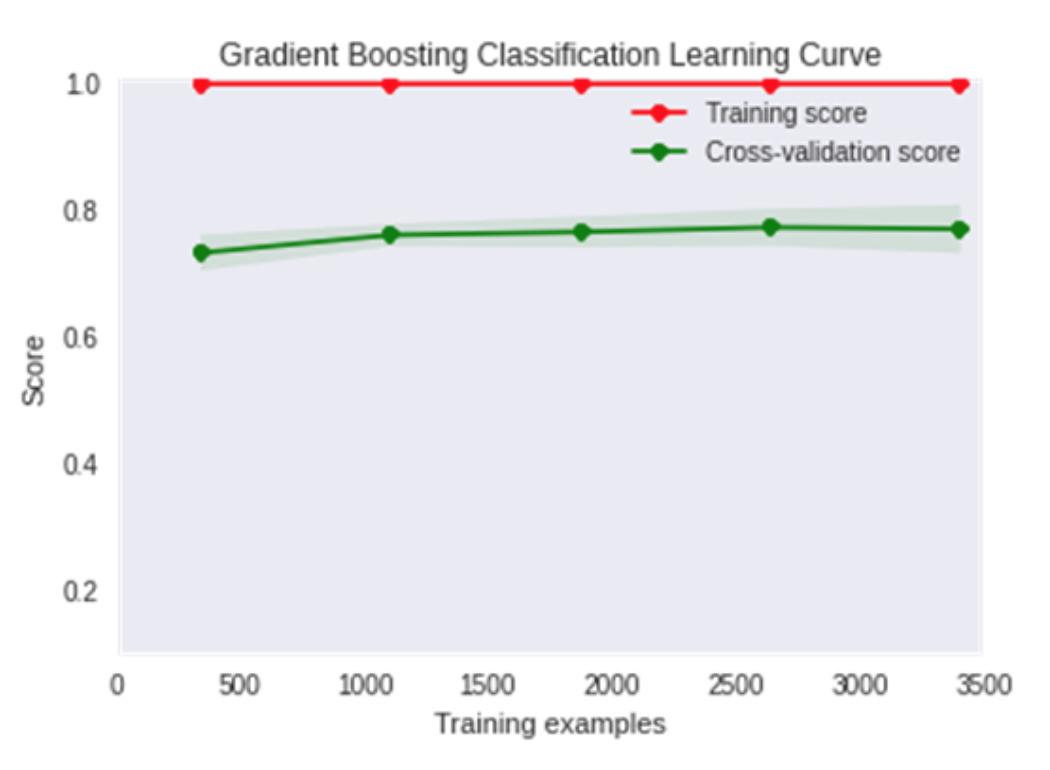
\includegraphics[width=3.2in]{figures/gb_learningcurve}
\caption{GB Learning curve}
\label{fig:learningcurve}
\end{figure}

Learning curve indicates the amount of data necessary to train a model up its maximal capability. It can be seen that Gradient Boosting Classifiers Requires over 3000
The analytical results coincide with findings of the parameters search over the pipeline ,which is \begin{verbatim}(max_leaf_nodes = None, learning_rate = 0.1,
max_depth =  10, min_samples_leaf = 5, 
max_features = 0.01, subsample = 1.0) \end{verbatim}­ This model has a good bias/variance balance, which produces a well generalising model.

\subsection{Final Model}
Two architectures were tested for the final model of unification of classification and regression results. To optimize the model, a custom GridsearchCV function was written in order to support two models in a pipeline and not just one which is default in Sklearn.
The second model performed worse, due to much smaller training data available and as it was seen before, gradient boost regression require over 3000 samples to achieve validation saturation.
\begin{figure}[h]
\centering
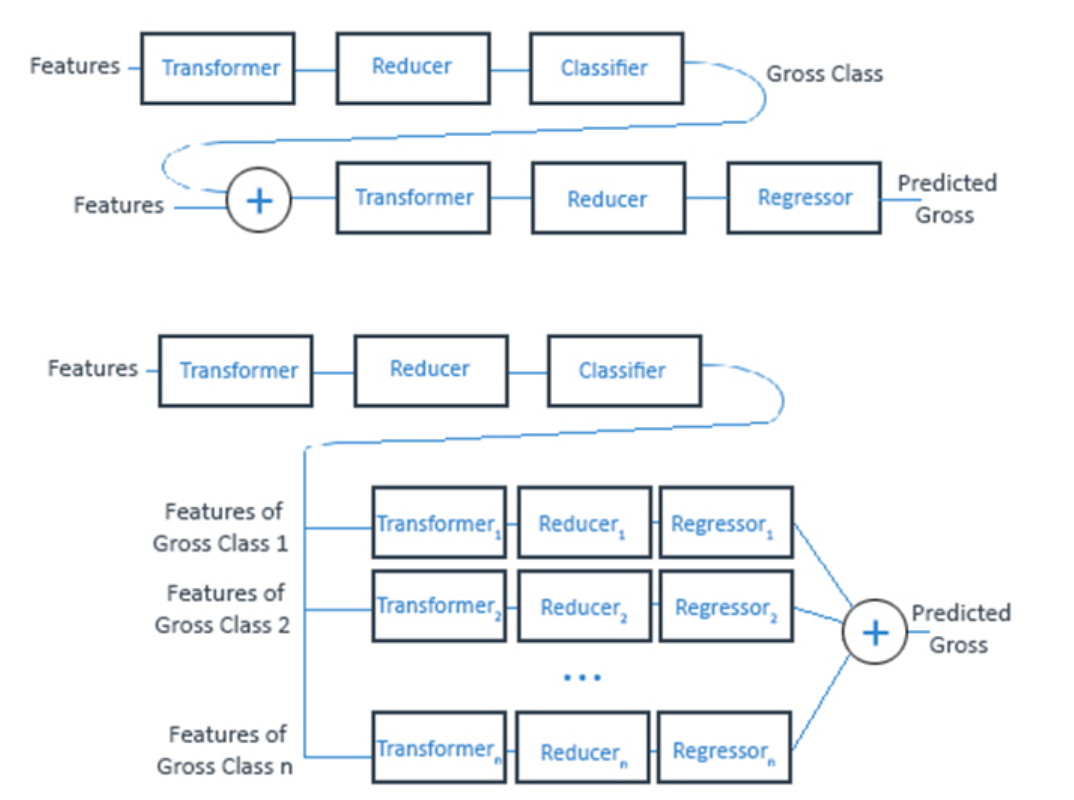
\includegraphics[width=3.2in]{figures/final_model}
\caption{Final model}
\label{fig:finalmodel}
\end{figure}

\section{Results}
\blindtext[2]
\section{Discussion}
\blindtext[2]
\section{Conclusion}
\blindtext[1]